% \question{questions are in red}

% \new{new text is purple}

% \ggd{Greg's comments look like this}

% \greg{New text written or modified by Greg in this color violet}


Modern observational astronomy has shown us that the Universe is not static and immutable: to the contrary, it is a lively and dynamic system. We now know and understand a variety of different phenomena that can give rise to variations in the brightness and color of astrophysical objects, including explosive stellar death (supernovae, kilonovae, Gamma Ray Bursts, etc), less dramatic and powerful stellar variability (flares, pulsations), and variability arising from geometric effects (such as planetary transients and microlensing). The time scales for these phenomena range from seconds to years. When the variations are terminal –like supernovae– or stochastic –like stellar flares– they are referred to as ``transients''. 
Detecting optical astrophysical transients characteristically requires sequences of images across a significant temporal baseline. Surveys like the Dark Energy Survey \citep[DES]{DES} or the future Rubin Observatory Legacy Survey of Space and Time \citep[LSST]{lsst} search for spatially localized changes in brightness in patches of sky previously observed. 

Due to the rarity of astrophysical transients, a long baseline in conjunction with the observation of a large area of the sky is typically required to detect a statistically significant sample of transients like supernovae and individual examples of rare events, such as kilonovae.  The process itself is arduous and requires considerable human intervention at multiple stages. The first step is typically the creation of high quality templates of each region of the sky that is to be searched; the templates are then subtracted from nightly images, a process known in astrophysics as Difference Image Analysis (DIA) that was initially pioneered by \cite{Tomaney_1996} and then formalized by \cite{Alard_1998} and there is a rich history of subsequent improvements in the efficiency and accuracy of DIA models. Templates  (\temp) are typically constructed as stacks of high quality (favorable observing conditions) sky images. These high quality images must then be aligned with the ``today'' image, typically called the ``search image'' (\search), and degraded to match its Point Spread Function (PSF, which we note may vary across a single large field of view image) and scaled to match its brightness. The product generated by the subtraction of the template from the search image is the so-called ``difference image''   (\diff; see for example a description of the DIA processing pipeline for DES in \citealt{Kessler_2015}).
Transients can then be detected as clusters of adjacent pixels deviating significantly from the sky noise.
% The current way of classifying optical images is to construct the image called template, which, in the case of  uses (READ \cite{Kessler_2015}), then the difference image is the residual obtained by subtracting the template and the science images. Many problems behind this steps to get the final classification and taking into account the large amount of data collected every day, the process of labeled objects by human inspection turns out to be very inefficient.))))\\
% Furthermore, miss-classifications due to human or computational error could lead to miss new astrophysical objects. \\
However, even the best existing DIA algorithms produce difference images with large pixel value deviation from an ideal 0-average that would be expected if no changes occurred in a patch of sky. Transients, variable stars, and moving objects will result in detections, but also a typically large number of artifacts will be detected by these thresholding schemes.

 

Machine learning models offer an excellent opportunity to improve the efficiency of transient detection at this stage, automating the classification between ``real'' astrophysical transients and ``bogus'' artifacts: these models are often referred to as ``Real-Bogus'' (hereafter, RB). Generally, the applications of machine learning to this problem are based on the extraction of features from the (difference) images that are then fed to models like Random Forests, k-Nearest Neighbors, or Support Vector Machines \citep{Goldstein_2015, S_nchez_2019, Mong_2020}. These models have achieved high accuracy and enabled the discovery of transients at scale in larger synoptic surveys, for example in the Palomar Transient Factory \citep[PTF][]{bloom2012automating} and Zwicky Transient Facility \citep[ZTF][]{2019PASP..131c8002M}. 

The process of engineering features for machine learning models allows the experts to embed domain knowledge in models. In the case of RB classification, the features engineered to be used by models such as the ones described above usually rely on visual inspection of a subset of the data. However, these features may overlook abstract associations between image properties that can be effective for classification, and in fact, may be biased towards human perception and theoretical expectations. An alternative approach involves the use of models that can learn features directly from the data, such as Convolutional Neural Networks \citep[CNNs]{lecun1989generalization}.  Here, it is possible to train a model using the images themselves, skipping the step of feature-design entirely.

RB CNN-based models appeared in the literature as early as 2016 \citep{Cabrera_2016}, and they are typically based on the analysis of the difference images arising from the DIA. While neural networks may be computationally demanding in the training phase, the "feed-forward" classification that arises from a pre-trained model is typically rapid and computationally light,\footnote{although the model may require a large amount of memory to cache.} leaving DIA as the computational bottle-neck in the process of astrophysical transients' detection. Yet in principle, the entirety of the information content embedded in the \diff-\temp-\search\ image triplet is also contained in the \temp-\search\ image pair.  In this paper, we explore the use of CNNs as RB models %(models that separate ``real'' astrophysical transients from ``bogus'' artifacts), 
concentrating on the potential for building high-accuracy models that \textit{do not} require the construction of difference images.  

 This paper represents a first, critical step in the process of conceptualizing and realizing a DIA-free model for astrophysical transients. Here we demonstrate that Neural Networks can discriminate between astrophysical transients and artifacts without a difference image, while still relying on DIA for detection. This is the necessary premise for the complete elimination of DIA and, with this conclusion in hand, in future work we intend to develop models that will not rely on DIA for detection, and, finally, that will detect and characterize transients (measure magnitude) from the \temp-\search\ image pair only.

% \subsection{Template}

% \subsection{Difference image analysis}

% \subsection{Convolutional Neural Network}

% SHOR DESCRIPTION ??

% In this paper we compare two CNN models trained on the same DES Y1 data \citep{Goldstein_2015}, one using as input data the template, search, and difference images, and the other using only the template and the search images. The main purpose is to demonstrate that relative simple CNN models are able to classify as ``real'' and ``bogus'' with high accuracy transient observations, without the necessity of the difference image.In \autoref{stateofart} we discuss the history, approaches, and details of DIA in the literature, and in \autoref{sec:data} we present the DES data that we will use to build our ``real''/``bogus'' classification models.  In \autoref{sec:results} we show the results of building a model that does not use the difference image as input and compare its performance to one that does, and we conclude with a discussion of the broader implications for this work in light of upcoming surveys in \autoref{sec:conclusion}.\\ 

This paper is organized as follows: in \autoref{sec:intro}, the introduction, we briefly describe DIA process, examples of architectures, and input images for CNNs models on the literature and describe the importance of our work. In \autoref{stateofart} we discuss the history, approaches, and details of DIA in the literature. In \autoref{sec:data} we present the DES data that we will use to build our RB classification models and the pre-processing steps. In \autoref{sec:method} we presented some general aspects of CNN and illustrate the CNNs architectures used, in \autoref{subsec: saliency} we present, share and discuss in some insights into the model obtained enabled by saliency maps, as well as the method used to interpret the data decisions through saliency maps. In \autoref{sec:results} we show the results of building a model that does not use the difference image as input, named \nodia -based model and compare its performance to one that does, named \diabased\ model;  we outline future work in \autoref{sec:futurework} and we conclude with a discussion of the broader implications for this result in light of upcoming surveys.

This study is reproducible and all the code that supports the analysis presented here is available on a dedicated \texttt{GitHub} repository. \footnote{\url{https://github.com/taceroc/DIA_noDIA}.}
% in \autoref{sec:conclusion}.
\begin{figure*}

    \centering
    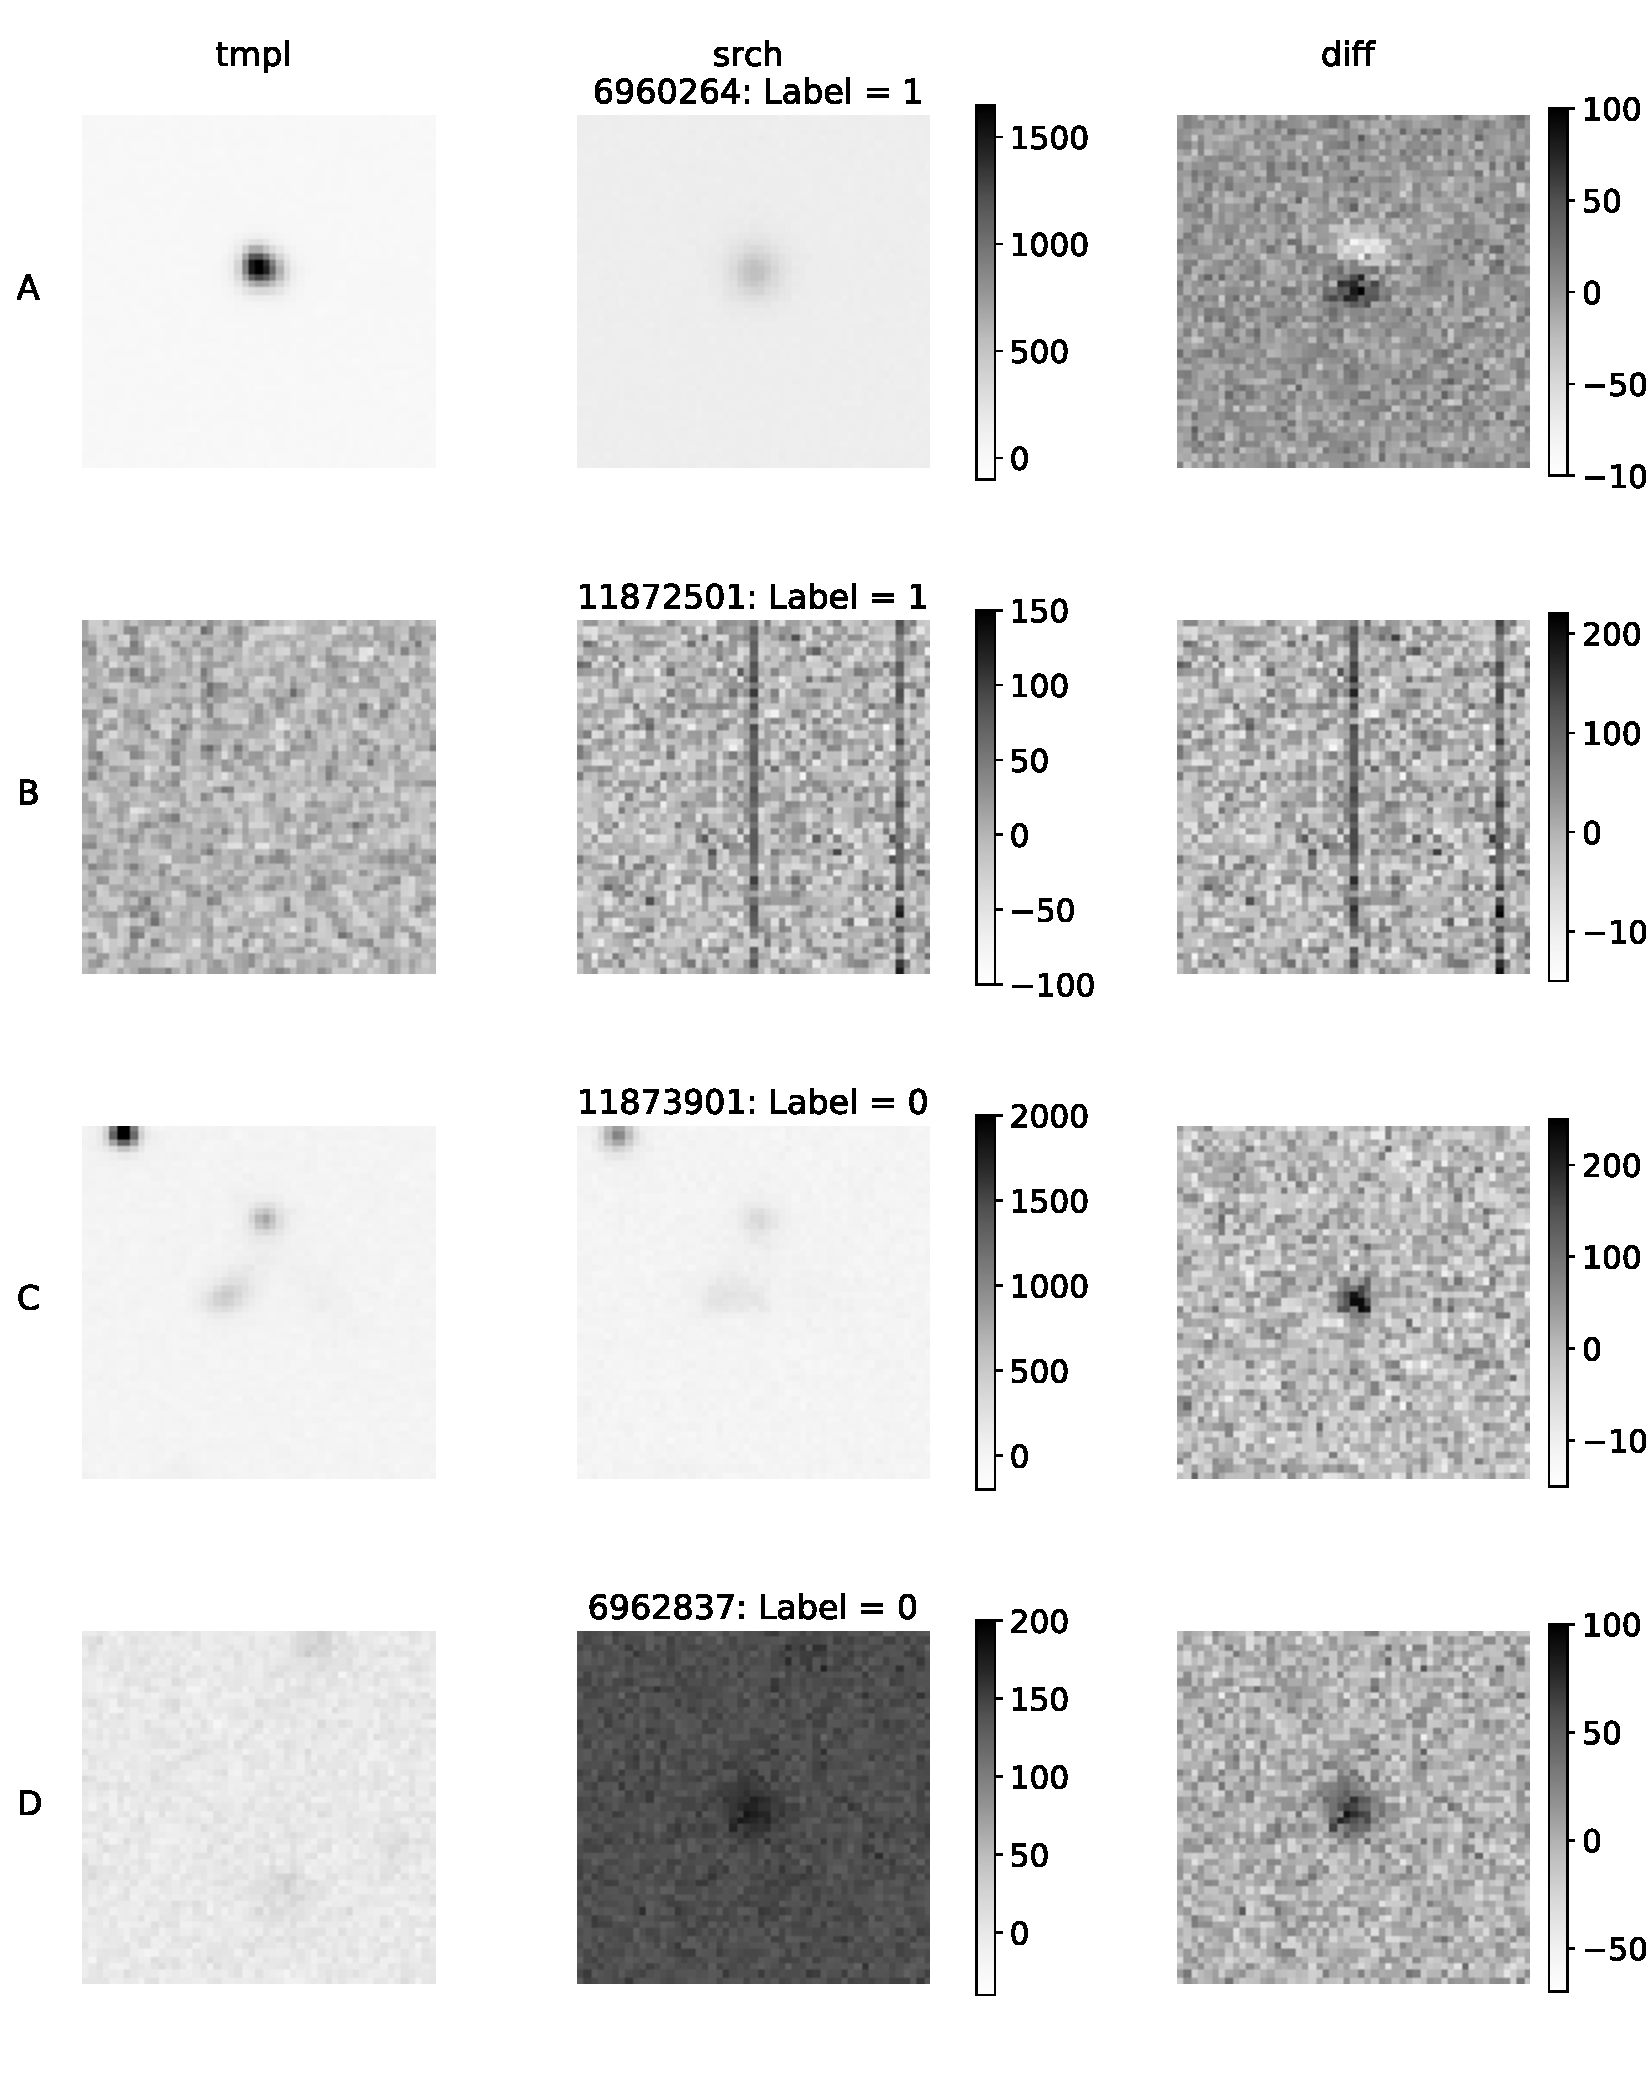
\includegraphics[width=0.52\linewidth]{figures/nonorm_new_test.pdf}
    \caption{Example of four DIA-sets from the first season of the Dark Energy Survey (DES): from left to right the images correspond to the template (\temp), search (\search), and difference (\diff) image; the \diff\ is generated as the subtraction of \temp\ and \search. Each pair of \temp\ and \search\ images is mapped to the same color range. We refer to these 3-images sets as ``image triplets'' or DIA-sets. A and B show artifacts, human-labeled as ``bogus'' (\texttt{label = 1}). C and D show transients labeled as ``real'' (\texttt{label = 0}).
     Above each triplet is the unique ID of the transient (see \citealt{Goldstein_2015})
    }
    \label{fig:examples_no_normalization}
\end{figure*}

%  in \autoref{sec:DI} we describe in more detail the Difference Imaging processes, in \autoref{sec:autoscan} we present relevant information about the precursor of our work \citep{Goldstein_2015},
\begin{figure*}
    \centering
    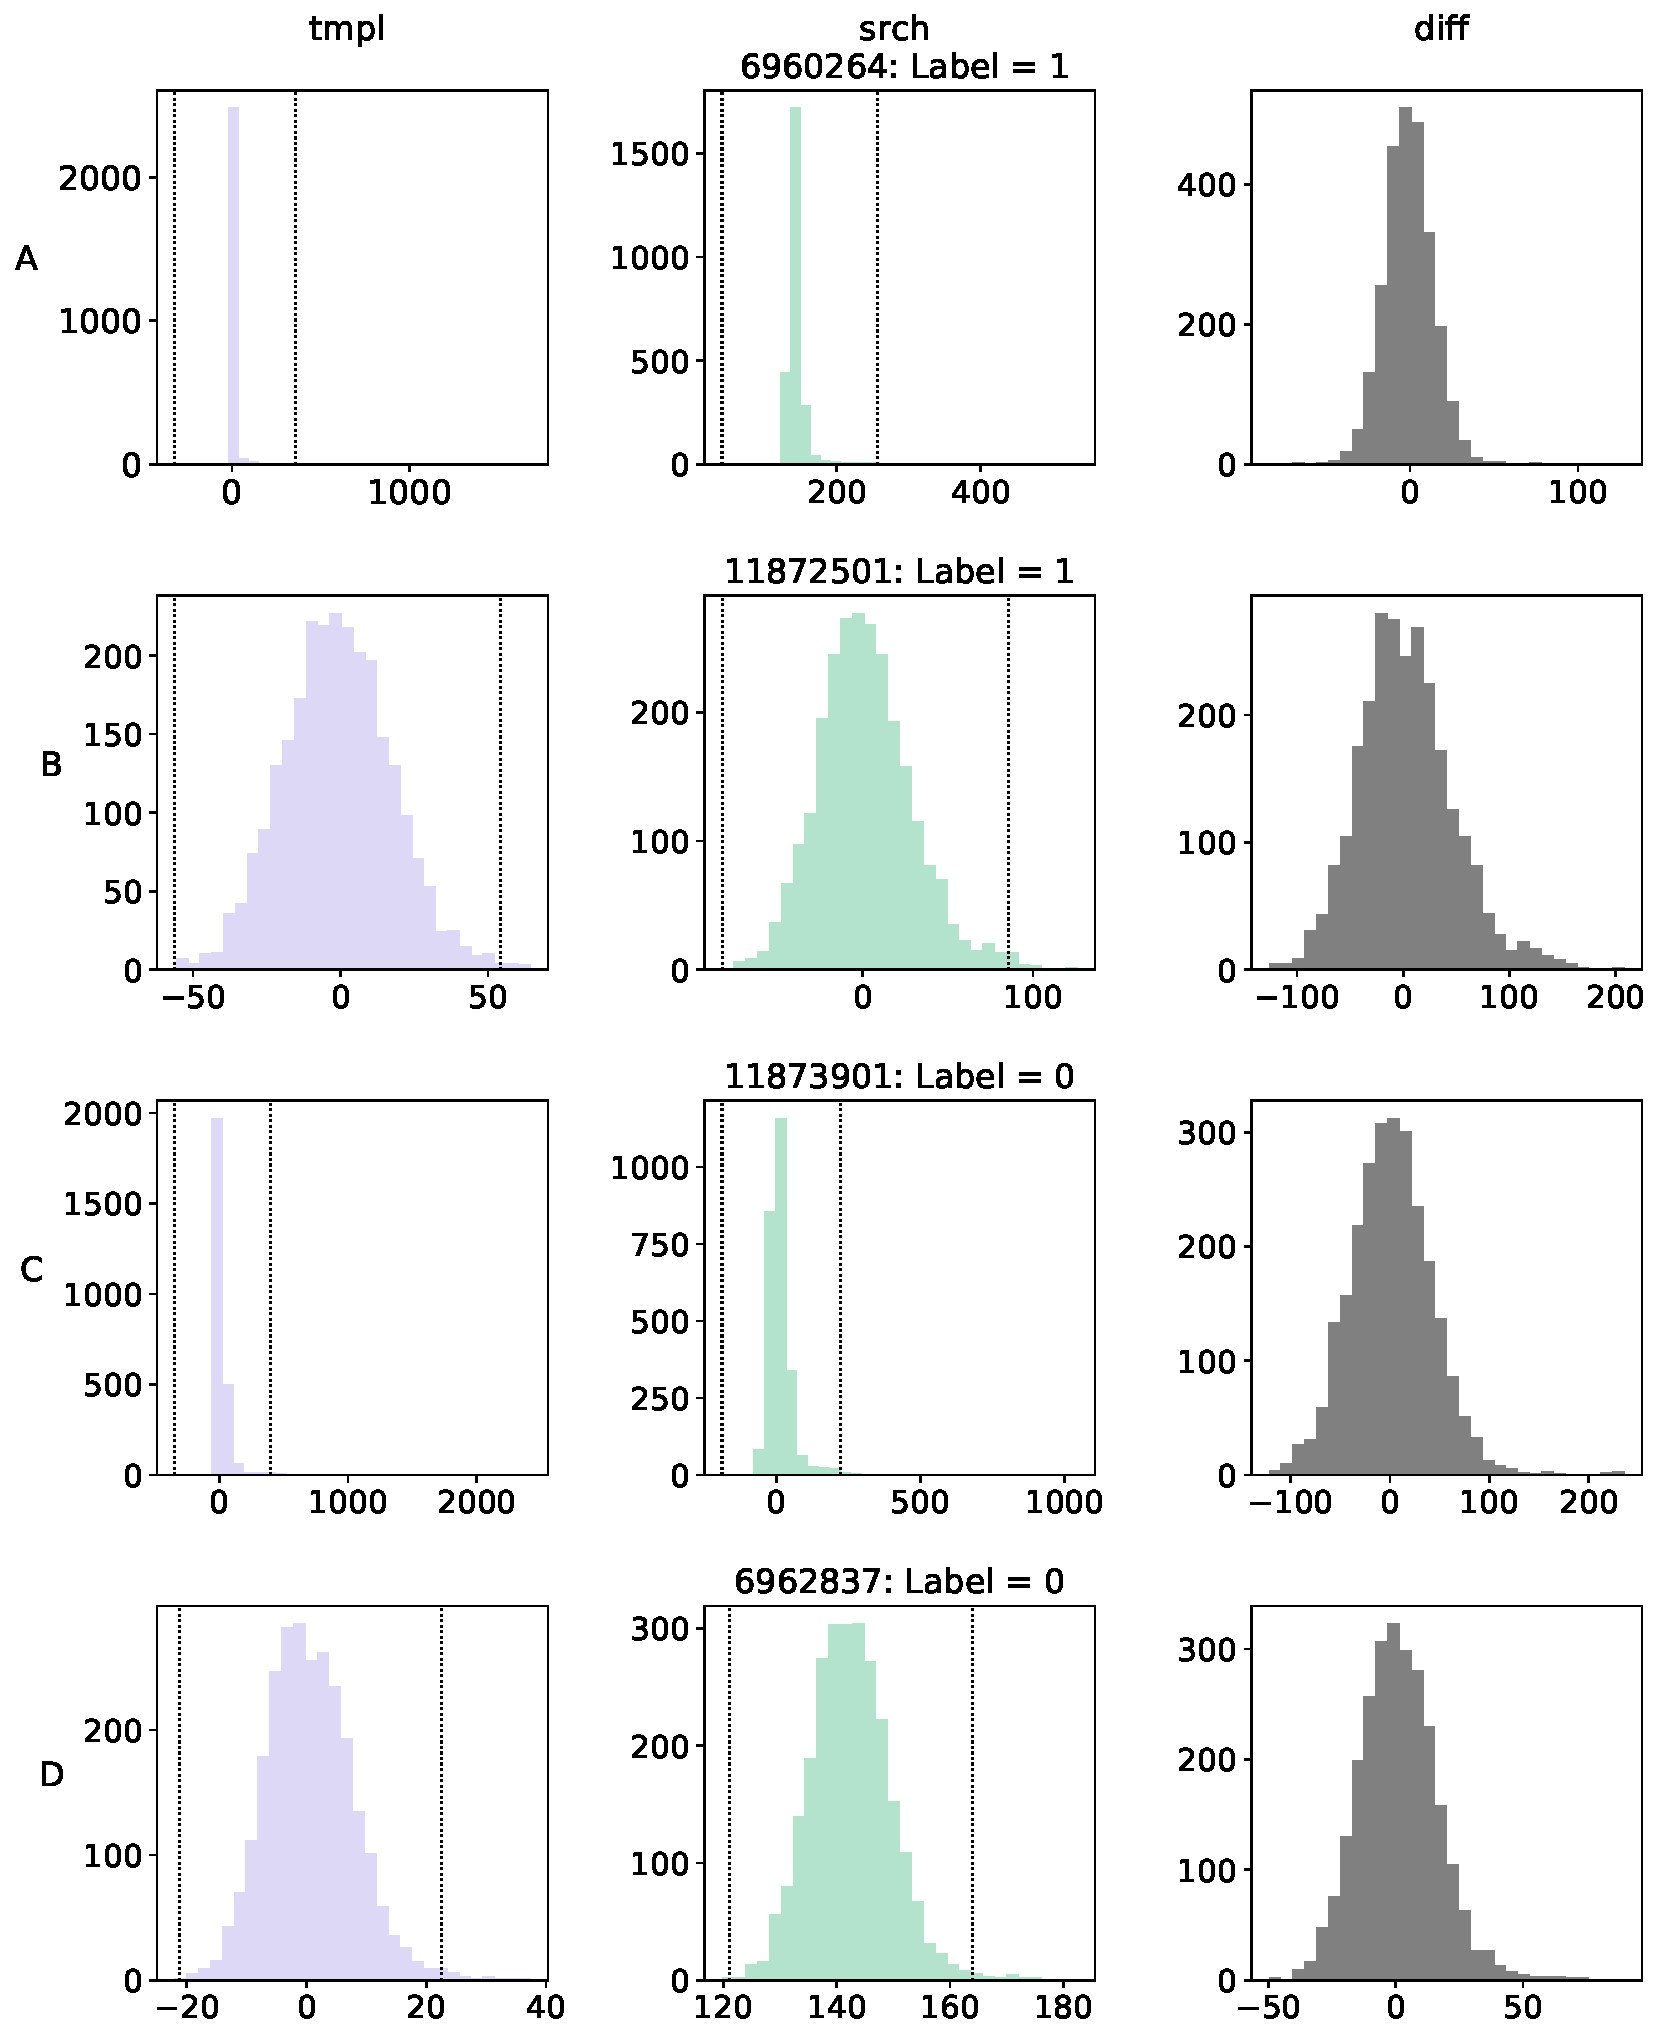
\includegraphics[width=0.6\linewidth]{
    figures/histnonorm_new_test_colors.pdf}
    \caption{Histogram of pixel values for %Quantitative representation of 
    the data shown in \autoref{fig:examples_no_normalization} (before scaling and normalization). 
    While all difference images (right) show bell-shaped distribution, the template and search image in both ``bogus'' and ``real'' sets have different behaviours. For example, B and D have similar pixel values distribution, however, B is ``bogus'' and D is ``real''. The vertical lines show the $\mu \pm 3\sigma$ interval for the \search\ and \temp\ images. The \diff\ images (last right column) are standardized individually to a mean of $0$ and a standard deviation of $1$. The \search\ and \temp\ are instead scaled, setting the pixel contained inside the 3$\sigma$ interval (vertical lines on the histograms) to the range 0-1. This allows to retain negative values or as well values above $1$ while keeping the core of the distributions to within a homogeneous range.
               }
    \label{fig:histobeforenormalizarion}
\end{figure*}


\begin{figure*}
    \centering
    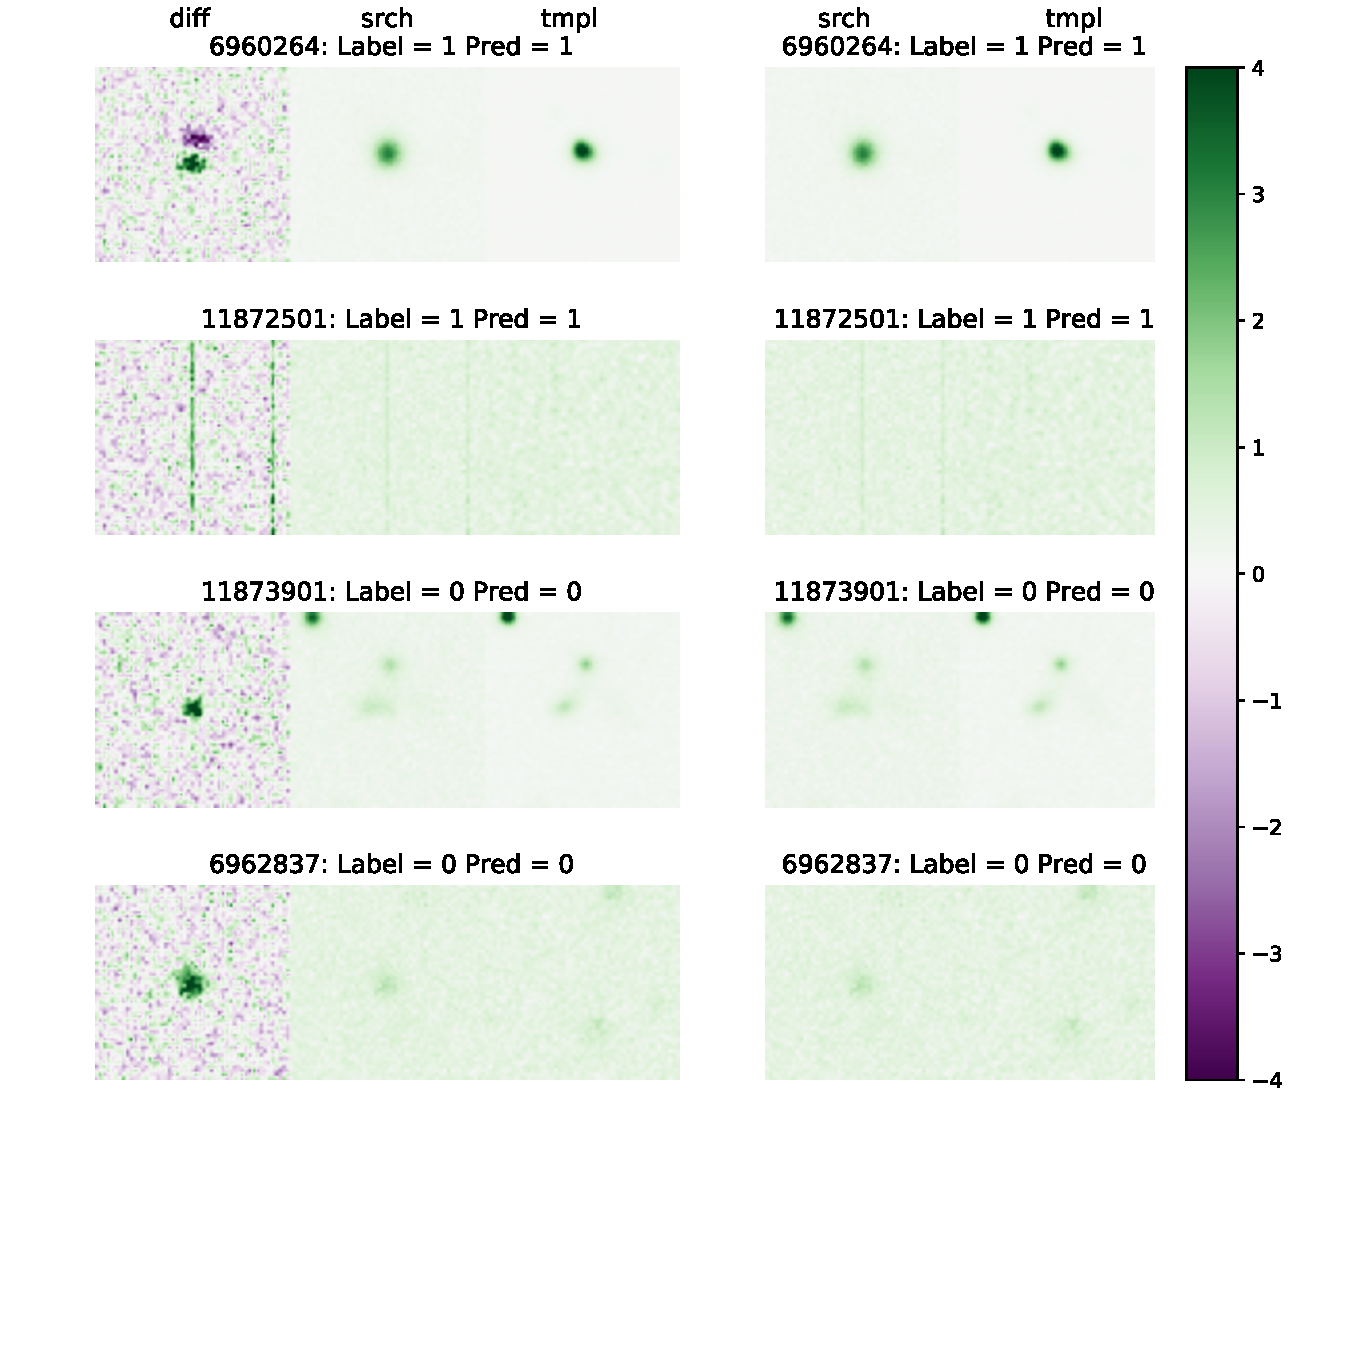
\includegraphics[width=0.7\linewidth]{
    figures/32dex_new_test.pdf}
    \caption{Horizontally stacked data for the examples shown in \autoref{fig:examples_no_normalization}. On the {\it left}, the composite images used as input to the \diabased\ CNN model: the composite follows the order, from left to right: \diff, \search, \temp. On the {\it right}, the composite images used for the \nodia\ model, composed of \search\ and \temp. Each images element was scaled or normalized following the description given in \autoref{sec:data} and \autoref{fig:histobeforenormalizarion} before combining them into a single image. Above each composite are the unique transient ``ID'', the original label, and prediction made by our model. The four transients were classified correctly by both \diabased\ and \nodia\ models. Purple shades indicate negative and green  positive pixel values.
%     \underline{Left}: Horizontally stacked normalized data for the examples shown in \autoref{fig:examples_no_normalization}. The stacked follow the order, from left to right: (\diff, \search, \temp). Each composite images is normalized as follows, the \diff\ are standarized (subtracting the mean and dividing by the standard deviation); \search\ and \temp\ are preprocessed using the min-max scheme. This is the format of the data input in the neural network (see section \ref{subsection: model_neural_network}).
% \underline{Right}: Horizontally stacked normalized data for the examples shown in \autoref{fig:examples_no_normalization}. The stacked follow the order, from left to right: (\search, \temp). Each composite images is normalized as follows, \search\ and \temp\ are preprocessed using the min-max scheme. This is the format of the data input in the neural network (see section \ref{subsection: model_neural_network}). The divergent color map used is \texttt{PRGn}, given by python
}
    %The color map used is ``viridis'', given by python. This images are the final data used for the Neural Network model.  }
    \label{fig:examples_hstack_normalization}
\end{figure*}
